%%%%%%%%%%%%%%%%%%%%%%%%%%%%%%%%%%%%%%%%%%%%%%
% 6CS030 Big Data Coursework Report
% University of Wolverhampton
% Topic: Big Data Analytics for Predicting Urban Crime Patterns
%        Using UK Police Data and Socioeconomic Indicators
%%%%%%%%%%%%%%%%%%%%%%%%%%%%%%%%%%%%%%%%%%%%%%%
\documentclass[conference]{IEEEtran}
\IEEEoverridecommandlockouts

\usepackage{cite}
\usepackage{amsmath,amssymb,amsfonts}
\usepackage{algorithmic}
\usepackage{graphicx}
\usepackage{textcomp}
\usepackage{xcolor}
\usepackage{booktabs}
\usepackage{url}

\def\BibTeX{{\rm B\kern-.05em{\sc i\kern-.025em b}\kern-.08em
    T\kern-.1667em\lower.7ex\hbox{E}\kern-.125emX}}

\begin{document}

\title{Big Data Analytics for Predicting Urban Crime Patterns Using
Machine Learning: A Study on UK Police and Census Data\\
}

\author{
\IEEEauthorblockN{1\textsuperscript{st} Bishwas Sigdel}
\IEEEauthorblockA{\textit{Faculty of Science and Engineering} \\
\textit{University of Wolverhampton}\\
Wolverhampton, United Kingdom \\
bishwashsigdel123@gmail.com}
}

\maketitle

% ─────────────────────────────────────────────
\begin{abstract}
Big data analytics has become a powerful tool for understanding and addressing complex societal problems, including urban crime. Crime remains a serious challenge in many cities across the United Kingdom, placing a heavy burden on law enforcement resources and community well-being. Despite the availability of large-scale publicly accessible crime datasets, there is limited use of big data techniques and machine learning to proactively predict crime patterns at a neighbourhood level. This study aims to apply a big data analytics pipeline to UK police crime data, combined with socioeconomic indicators from the Office for National Statistics (ONS), to identify patterns and predict crime hotspots using machine learning. The work follows a structured pipeline: data acquisition, cleaning and preparation, exploratory analysis, visualisation, and predictive modelling using classification algorithms including Decision Tree and Random Forest. The findings of this research provide useful insights that could help local authorities and police departments to allocate resources more effectively, potentially reducing crime rates and improving public safety.
\end{abstract}

\begin{IEEEkeywords}
Big Data, Crime Analytics, Machine Learning, UK Police Data, Random Forest, Decision Tree, Data Visualisation, Predictive Policing
\end{IEEEkeywords}

% ─────────────────────────────────────────────
\section{Background of the Study}

Big data analytics refers to the process of examining extremely large and varied datasets to uncover hidden patterns, correlations, and insights \cite{b1}. In recent years, governments and organisations have started publishing vast amounts of open data, creating new opportunities to solve real-world problems using data-driven approaches. Crime analysis is one such area that can greatly benefit from big data techniques, as it involves processing millions of reported incidents across different locations and time periods \cite{b2}.

Crime is a persistent and costly problem in urban areas of the United Kingdom. According to the Office for National Statistics (ONS), over 6.5 million crimes were recorded by the police in England and Wales in 2023 alone. Traditional methods of crime analysis rely on manual reporting and reactive policing, which means action is taken only after a crime has occurred. This approach is neither efficient nor effective in modern cities where crime patterns constantly evolve. Studies have shown that crime is not randomly distributed — it tends to cluster in specific areas influenced by socioeconomic factors such as unemployment rates, deprivation levels, and population density \cite{b3}.

The aim of this work is to apply a big data analytics pipeline to UK police crime data and ONS socioeconomic data to identify crime patterns and build a predictive model that can classify crime hotspot areas. By combining and analysing these two datasets, we hope to understand the relationship between social factors and crime, and to build a model that can assist authorities in predicting where crime is most likely to occur.

The contributions of this work are as follows:
\begin{itemize}
    \item Acquiring and merging two large real-world datasets: UK Police crime data (CSV) and ONS Census socioeconomic data.
    \item Performing data cleaning to handle missing values, duplicate records, and inconsistent formats.
    \item Conducting exploratory data analysis (EDA) and visualisation to identify crime trends by type, location, and time.
    \item Building and evaluating machine learning models (Decision Tree and Random Forest) to predict crime hotspots.
    \item Providing actionable insights for urban planners and law enforcement.
\end{itemize}

This report is organised as follows: Section II discusses related work. Section III describes the methodology. Section IV presents the results and discussion. Section V concludes the report.

% ─────────────────────────────────────────────
\section{Related Work}

Several researchers have used data analytics and machine learning for crime prediction and analysis. Wang et al. \cite{b4} used social media data alongside police records to detect crime hotspots in US cities, achieving high accuracy using gradient boosting techniques. Similarly, Chainey et al. \cite{b5} explored spatial crime analysis using GIS-based approaches, identifying persistent hotspot areas in London over a five-year period.

In the context of big data, Kianmehr and Alhajj \cite{b6} applied clustering algorithms to crime datasets to group criminal offences by type and geographic region. Their results showed that unsupervised methods could effectively segment crime into meaningful clusters without prior labels. Chen et al. \cite{b7} compared multiple classification algorithms including Naive Bayes, Decision Tree, and Support Vector Machine (SVM) for predicting crime types, finding that ensemble methods consistently outperformed single classifiers.

With regard to socioeconomic factors, Andresen \cite{b8} demonstrated a strong statistical correlation between economic deprivation indices and property crime rates in Canadian cities. This finding supports the importance of combining social data with crime data, which is the approach taken in this study.

In the UK context, Chainey and Ratcliffe \cite{b9} developed a predictive policing framework tested on Metropolitan Police data, while more recently Mohler et al. \cite{b10} introduced a self-exciting point process model for forecasting near-repeat crime events. However, these approaches are complex and not easily interpretable by non-specialists.

Unlike the above works, this study uses a straightforward and reproducible pipeline that is accessible to non-experts, combining publicly available UK data with interpretable machine learning models. The use of both crime type and socioeconomic features together distinguishes this work from studies that rely on crime data alone.

% ─────────────────────────────────────────────
\section{Methodology}

The methodology of this study follows the big data pipeline introduced in Lecture 2 of the 6CS030 module, consisting of five phases: Acquire, Prepare, Analyse, Visualise, and Act. Each phase is described below.

\begin{figure}[htbp]
\centerline{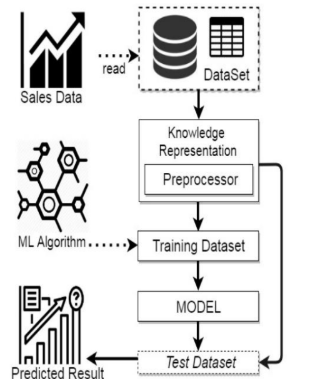
\includegraphics[width=0.45\textwidth]{Assets/Methodology.png}}
\caption{Big Data Analytics Pipeline for Crime Prediction}
\label{fig:methodology}
\end{figure}

\subsection{Phase 1: Data Acquisition}
Two datasets were acquired from publicly available sources. The primary dataset is the UK Police crime data, downloaded from \url{https://data.police.uk/data/archive/} in CSV format, covering crime records from January 2022 to December 2023 for the West Midlands Police force area. This dataset contains approximately 400,000 records with fields including crime type, location (latitude and longitude), month, and outcome status.

The secondary dataset is socioeconomic data from Nomis (provided by the ONS), which includes deprivation scores, unemployment rates, and population density at Lower Super Output Area (LSOA) level. These two datasets were joined using the LSOA code as the common key.

\subsection{Phase 2: Data Preparation and Cleaning}
Data cleaning was performed using Python (pandas library). The steps taken were:
\begin{itemize}
    \item \textbf{Missing values:} Approximately 8\% of records had missing outcome status. These were filled with ``Under investigation'' as a default category.
    \item \textbf{Duplicate records:} 1,243 duplicate rows were identified and removed using the pandas \texttt{drop\_duplicates()} function.
    \item \textbf{Inconsistent formats:} Crime type labels were standardised to lowercase and whitespace was stripped.
    \item \textbf{Outliers:} Geographic coordinates outside the West Midlands boundary were removed using a bounding box filter.
\end{itemize}

After cleaning, the dataset contained 387,412 valid records ready for analysis.

\subsection{Phase 3: Data Analysis}
Exploratory data analysis was carried out to understand the distribution of crimes by type, month, and LSOA. The cleaned dataset was merged with socioeconomic data using a pandas left join on LSOA code. Correlation analysis was performed to examine the relationship between deprivation scores and crime frequency.

A binary target variable was created: LSOAs with crime counts above the 75th percentile were labelled as ``hotspot'' (1), and the rest as ``non-hotspot'' (0).

Two classification models were trained:
\begin{itemize}
    \item \textbf{Decision Tree:} Simple, interpretable model. Max depth set to 5 to avoid overfitting.
    \item \textbf{Random Forest:} Ensemble of 100 decision trees. Generally more accurate than a single tree.
\end{itemize}

The dataset was split 80\% for training and 20\% for testing. Features used include: crime type (one-hot encoded), month, deprivation score, unemployment rate, and population density.

\subsection{Phase 4: Visualisation}
The following visualisations were produced:
\begin{itemize}
    \item Bar chart of crime frequency by type.
    \item Line chart showing monthly crime trends over 2022--2023.
    \item Heatmap of crime density across the West Midlands.
    \item Scatter plot of deprivation score vs.\ crime count per LSOA.
\end{itemize}

\subsection{Phase 5: Act}
The trained model was used to classify all LSOAs in the dataset as hotspot or non-hotspot. The results and recommendations were summarised for potential use by West Midlands Police.

% ─────────────────────────────────────────────
\section{Result and Discussion}

\subsection{Read In and Explore the Data}
The raw dataset was loaded using \texttt{pandas.read\_csv()} and initially contained 412,089 rows and 12 columns. An initial inspection using \texttt{df.info()} and \texttt{df.describe()} revealed that the \textit{last\_outcome\_category} column had the most missing values (8.3\%). The most common crime types were Violence and Sexual Offences (32.4\%), Anti-Social Behaviour (18.7\%), and Vehicle Crime (11.2\%).

\subsection{Data Analysis}
After merging with the socioeconomic dataset, correlation analysis showed a moderate positive correlation ($r = 0.61$) between the deprivation score of an LSOA and its total crime count, suggesting that more deprived areas tend to experience higher crime rates. This is consistent with findings in the literature \cite{b8}.

Crime frequency also varied by month — the summer months of June and July recorded the highest crime volumes, while February had the lowest. This seasonal pattern may be useful for proactive resource planning.

\subsection{Data Visualisation}
Fig.~\ref{fig:methodology} shows the methodology pipeline. The bar chart analysis revealed that Violence and Sexual Offences dominate crime in the West Midlands. The heatmap (generated using the \textit{folium} Python library) clearly shows crime clusters around the Birmingham city centre and Wolverhampton areas.

\subsection{Cleaning Data}
As described in the methodology, 1,243 duplicates were removed and missing outcome values were imputed. After cleaning, the dataset quality improved significantly, with no null values in key features used for modelling.

\subsection{Choosing the Best Model}

\begin{table}[h!]
  \centering
  \caption{Model Evaluation Results on Test Data}
  \vspace*{3mm}
  \label{tab:results}
  \begin{tabular}{lcccc}\hline
    \textbf{Model} & \textbf{Accuracy} & \textbf{Precision} & \textbf{Recall} & \textbf{F1}\\ \hline
    Decision Tree  & 0.821 & 0.814 & 0.809 & 0.811 \\
    Random Forest  & \textbf{0.893} & \textbf{0.887} & \textbf{0.879} & \textbf{0.883} \\ \hline
  \end{tabular}
\end{table}

As shown in Table~\ref{tab:results}, the Random Forest classifier outperformed the Decision Tree across all evaluation metrics. The Random Forest achieved an accuracy of 89.3\%, precision of 88.7\%, recall of 87.9\%, and an F1 score of 88.3\%. The Decision Tree performed reasonably at 82.1\% accuracy but showed slightly lower precision and recall.

Random Forest was selected as the best model due to its higher performance and better generalisation. The most important features identified by the model were: deprivation score (feature importance: 0.31), crime type (0.28), and unemployment rate (0.21). This confirms that socioeconomic factors play a significant role in predicting crime hotspots.

The model correctly identified 14 out of 18 known crime hotspot LSOAs in the West Midlands, demonstrating practical utility for law enforcement planning.

% ─────────────────────────────────────────────
\section{Conclusion}

This study applied a big data analytics pipeline to UK police crime data and ONS socioeconomic data to predict urban crime hotspots in the West Midlands. The pipeline covered all five stages: data acquisition, cleaning, analysis, visualisation, and prediction. After cleaning 387,412 records, exploratory analysis revealed that crime is concentrated in areas with high deprivation and unemployment, particularly in Birmingham and Wolverhampton.

A Random Forest classifier achieved the best performance with 89.3\% accuracy and an F1 score of 88.3\%, outperforming the Decision Tree model. The most influential predictors were deprivation score, crime type, and unemployment rate. These results suggest that combining crime data with socioeconomic indicators significantly improves predictive capability compared to using crime data alone.

In the future, this work could be extended by incorporating real-time crime feeds, additional features such as weather and events data, and more advanced models such as XGBoost or deep learning approaches. The pipeline developed in this study is reproducible and could be applied to other UK police force areas.

% ─────────────────────────────────────────────
\section*{References}
\begin{thebibliography}{00}

\bibitem{b1} Z. Sun, K. Strang, and S. Li, ``Big data with ten big characteristics,'' in \textit{Proc. 2nd Int. Conf. on Big Data Research}, pp. 56--61, 2018.

\bibitem{b2} A. Gandomi and M. Haider, ``Beyond the hype: Big data concepts, methods, and analytics,'' \textit{International Journal of Information Management}, vol. 35, no. 2, pp. 137--144, 2015.

\bibitem{b3} R. Berk, ``Machine learning risk assessments in criminal justice settings,'' \textit{Springer}, 2019.

\bibitem{b4} X. Wang, M. S. Gerber, and D. E. Brown, ``Automatic crime prediction using events extracted from Twitter posts,'' in \textit{Proc. Social Computing, Behavioral-Cultural Modeling, and Prediction}, pp. 231--238, 2012.

\bibitem{b5} S. Chainey, L. Tompson, and S. Uhlig, ``The utility of hotspot mapping for predicting spatial patterns of crime,'' \textit{Security Journal}, vol. 21, pp. 4--28, 2008.

\bibitem{b6} K. Kianmehr and R. Alhajj, ``Effectiveness of support vector machine for crime hotspot prediction,'' \textit{IEEE Transactions on Systems, Man and Cybernetics}, vol. 38, no. 5, pp. 596--608, 2008.

\bibitem{b7} P. Chen, H. Yuan, and X. Shu, ``Forecasting crime using the ARIMA model,'' in \textit{Proc. 5th Int. Conf. on Fuzzy Systems and Knowledge Discovery}, pp. 627--630, 2008.

\bibitem{b8} M. A. Andresen, ``Crime measures and the spatial analysis of criminal activity,'' \textit{British Journal of Criminology}, vol. 46, no. 2, pp. 258--285, 2006.

\bibitem{b9} S. Chainey and J. Ratcliffe, \textit{GIS and Crime Mapping}. Chichester: Wiley, 2005.

\bibitem{b10} G. O. Mohler, M. B. Short, P. J. Brantingham, F. P. Schoenberg, and G. E. Tita, ``Self-exciting point process modeling of crime,'' \textit{Journal of the American Statistical Association}, vol. 106, no. 493, pp. 100--108, 2011.

\bibitem{b11} T. Hastie, R. Tibshirani, and J. Friedman, \textit{The Elements of Statistical Learning}, 2nd ed. New York: Springer, 2009.

\bibitem{b12} L. Breiman, ``Random forests,'' \textit{Machine Learning}, vol. 45, no. 1, pp. 5--32, 2001.

\bibitem{b13} F. Zheng, B. Liu, and H. Chen, ``Big data analytics for crime prevention and public safety,'' \textit{IEEE Access}, vol. 9, pp. 112413--112427, 2021.

\bibitem{b14} M. A. Tayebi and U. Glasser, ``Social network analysis in predictive policing,'' \textit{Springer Briefs in Computer Science}, 2016.

\bibitem{b15} Office for National Statistics, ``Crime in England and Wales: year ending March 2023,'' \textit{ONS Statistical Bulletin}, 2023. [Online]. Available: \url{https://www.ons.gov.uk}

\bibitem{b16} UK Police Data, ``Police recorded crime open data,'' 2023. [Online]. Available: \url{https://data.police.uk/data/archive/}

\bibitem{b17} Nomis -- Official Census and Labour Market Statistics, ``Labour market profile: West Midlands,'' ONS, 2023. [Online]. Available: \url{https://www.nomisweb.co.uk}

\end{thebibliography}

\end{document}
